% ----------------------------------------------------------
% Apêndices
% ----------------------------------------------------------

\chapter{Conceitos matemáticos}
\label{ap:conceitos_matematicos}

Neste capítulo iremos abordar alguns conceitos matemáticos importantes para o entendimento deste trabalho.

\section{Aritmética modular}
    A aritmética modular é um dos conceitos estudados pelo ramo da matemática conhecido como teoria dos números, que será amplamente utilizado neste trabalho. O conhecimento de aritmética modular será necessário para compreender alguns problemas de criptografia abordados nos Capítulo \ref{cap:criptografia} e \ref{cap:lattice_problems}. O algoritmo \ac{ML-KEM} também faz o uso da aritmética modular nas operações aritméticas entre polinômios, na qual é vista com mais detalhes no Apêndice \ref{ap:abstract_algebra}.

\begin{definition}[divisibilidade]
 Sejam $a$ e $b$ inteiros diferentes de $0$, é dito que $a$ é divisível por $b$ se e somente se existe um inteiro $c$ tal que $a = b.c$, a notação usada para denotar essa divisibilidade de $a$ por $b$ é $a\:|\:b$.
 \end{definition}

\begin{theorem}
    Se $a\:|\:b$ e $a\:|\:c$, então $(b + c)\:|\:a$.
\end{theorem}

\begin{theorem}
    Se $a\:|\:b$, então $(a.c)\:|\:b$.
\end{theorem}

\begin{theorem}
    Se $a\:|\:b$ e $b\:|\:c$, então $a\:|\:c$.
\end{theorem}

\begin{theorem}
Seja $n \in \mathbb{Z}$ e $d \in \mathbb{Z}_{+}$, existe um único par de inteiros $q$ e $r$ com $0 \leq r < d$ tais que $n = d.q + r$.
\end{theorem}

Sejam $n,d,q,r \in \mathbb{Z}$ tais que $d > 0$, $n = d.q + r$ e $0 \leq r < d$, definem-se as funções \textbf{div} e \textbf{mod} tais que:

\begin{itemize}
	\item $n$\ \textbf{div} $d = q$;
	\item $n$\ \textbf{mod} $d = r$.
\end{itemize}

\begin{definition}[Congruência modular]
Dados $j, k \in \mathbb{Z}$ e $m \in \mathbb{Z}_{+}$, é dito que $j$ é congruente a $k$ no módulo $m$ se e somente se $(j - k) \ |\  m$. A notação de congruência é $j \equiv k\ (\textbf{mod}\ m)$, ou seja, $j$ e $k$ são o mesmo número no módulo m.
\end{definition}

    \noindent
    \textbf{Propriedades da congruência modular}:
    \begin{itemize}
         \item \textbf{Propriedade reflexiva:} Seja $m \in \mathbb{Z}_{+}$, $n \equiv n\: (\textbf{mod}\: m)\: \forall n \in \mathbb{Z}$;
    	\item \textbf{Propriedade simétrica:} Seja $m \in \mathbb{Z}_{+}$, $j \equiv k\: (\textbf{mod}\: m)$ se e somente se $k \equiv j\: (\textbf{mod}\: m)$;
    	\item \textbf{Propriedade transitiva:} Seja $m \in \mathbb{Z}_{+}$, se $j \equiv k\: (\textbf{mod}\: m)$ e $k \equiv i\: (\textbf{mod}\: m)$ então $j \equiv i\: (\textbf{mod}\: m)$.
    \end{itemize}
    
    \begin{exemplo}
    para facilitar o entendimento sobre conceito de congruência, considere um relógio de 12 horas. Se agora são 5 horas, que horas serão daqui a 10 horas? Como este relógio não possui 15 horas, reinicia-se a contagem a partir de 0 quando o relógio chega em 12 horas. Dessa forma tem-se que 15 = 12 + 3; neste caso, se agora são 5 horas, daqui a 10 horas serão 3 horas. Desta forma é dito que $15 \equiv 3\ (\textbf{mod}\ 12)$, visto que $(15 - 3)\ |\ 12$.
    \qed
    \end{exemplo}

\pagebreak
\section{Teoria dos números}

    Esta seção apresenta alguns conceitos estudados no campo da teoria dos números mencionados na Seção \ref{sec:problemas_computacionais}, onde é abordado os problemas que os algoritmos de criptografia atuais são baseados.

    \begin{definition}[número primo]
        Um número natural maior que 1 que possui como divisores positivos apenas 1 e ele próprio.
    \end{definition}

    \begin{definition}[coprimos]
        Dois números são coprimos, ou primos entre si, se o único divisor comum entre eles for o número 1.
    \end{definition}

    \begin{exemplo}
        os divisores do número 4 são: 2 e 1, e os divisores do número 9 são: 3 e 1. Portando os números 4 e 9 são coprimos.
    \qed
    \end{exemplo}
   

    \begin{definition}[número composto]
        Dado $n,n_1,n_2 \in \mathbb{N}$ tal que $n > 1$, $n\ |\ n_1$ e $n\ |\ n_2$. Temos que $n$ é dito composto se $n = n_1 n_2$, com $1 < n_1 < n$ e $1 < n_1 < n$. 
    \end{definition}

    \begin{theorem}[teorema fundamental da aritmética]
        Todo número natural maior que 1 ou é primo, ou pode ser escrito como um produto de números primos.
    \end{theorem}

    Segundo o teorema fundamental da aritmética dado um número composto, por exemplo o número 145, podemos representá-lo pela multiplicação de números primos, neste caso 5 e 29. O problema da fatoração prima, abordado na Seção \ref{sec:problema_fatoracao_prima} utiliza este teorema.

    \begin{definition}[ordem multiplicativa]
        Dado os números inteiros positivos $n$ e $m$, tais que $n$ e $m$ são coprimos, a ordem multiplicativa de $n$ módulo $m$ é o menor valor inteiro positivo $k$ que satisfaz $n^k \equiv 1\ (\textbf{mod}\ m)$.
    \end{definition}

    \begin{exemplo}
        tem-se que \(2^6 \equiv 1\ (\textbf{mod}\ 7)\). No entanto, \(2^3 \equiv 1\ (\textbf{mod}\ 7)\). Observa-se que ambos satisfazem a congruência; porém, 3 é o menor expoente que satisfaz a equação. Portanto, conclui-se que 3 é a ordem multiplicativa de 2 módulo 7.
    \qed
    \end{exemplo}

    \begin{definition}[função totiente de Euler]
        A função totiente de Euler de um número natural $n$, denotada por $\varphi(n)$, é a quantidade de números coprimos a $n$ no intervalo $1 \le \varphi(n) < n$.
    \end{definition}

    \begin{exemplo}
         tem-se $\varphi(10) = 4$ pois a quantidade de números coprimos a 10 no intervalo ${[}1,10{[}$ é o conjunto $\{1, 3, 7, 9\}$ contendo 4 elementos.
    \qed
    \end{exemplo}

    \begin{definition}[raiz primitiva módulo m]
        Se a ordem multiplicativa de $k$ módulo $m$ é igual à função totiente de Euler para $m$, dizemos que $k$ é uma raiz primitiva módulo $m$.
    \end{definition}

    \begin{exemplo}
        é dito que 3 é uma raiz primitiva módulo 10, visto que a ordem multiplicativa de 3 e 10 é 4, e como calculado anteriormente, $\varphi(10) = 4$. Sendo assim, como a ordem multiplicativa entre 3 e 10 é igual à função totiente de 10, o número 3 é uma raiz primitiva módulo 10. Este conceito é utilizado no problema do logaritmo discreto, abordado na Seção \ref{sec:problema_logaritmo_discreto}.
    \qed
    \end{exemplo}

\pagebreak
\section{Álgebra linear}
Esta seção se dedica a alguns conceitos de álgebra linear essenciais para a compreensão deste trabalho. A álgebra linear é um ramo da matemática que se dedica no estudo de equações lineares, vetores, espaços vetoriais, matrizes, entre outros.

\begin{definition}[matriz]
    Chamamos de matriz $m \times n$ uma tabela de elementos dispostos em m linhas e n colunas.
\end{definition}

    \begin{center}
        $\textbf{A}_{m \times n} = \begin{bmatrix}
            a_{11} & a_{12} & . & . & . & b_{1n}\\
            a_{21} & a_{22} & . & . & . & b_{2n}\\
            a_{31} & a_{32} & . & . & . & b_{3n}\\
            .      & .      & . &   &   & .     \\
            .      & .      &   & . &   & .     \\
            .      & .      &   &   & . & .     \\
            a_{m1} & a_{m2} &   &   &   & a_{mn}
        \end{bmatrix}$
        %
        $= {[}a_{ij}{]}_{m \times n}$
    \end{center}

    O número de linhas e colunas é dito a ordem de uma matriz. É importante ressaltar algumas matrizes especiais, como a matriz quadrada, em que o número de linhas é igual o número de colunas; matriz nula, em que todos os elementos são zero, tal matriz é representada por \textbf{0}; matriz coluna, em que se tem apenas uma coluna e analogamente matriz linha, em que se tem apenas uma linha; por fim, matriz identidade quadrada, denotada por \textbf{I} tal que $a_{ii} = 1$ e $a_{ij} = 0$ para $i \neq j$.

    A seguir, é definida as operações e propriedades de soma entre matrizes de mesma ordem, multiplicação de uma matriz por um escalar, operação de transposição e multiplicação entre matrizes.
    
    A adição de matrizes de mesma ordem, isto é $\textbf{A}_{m \times n}$ + $\textbf{B}_{m \times n}$ é representada por:

                        $$\textbf{A} + \textbf{B} = {[}a_{ij} + b_{ij}{]}_{m \times n}$$
                
    \noindent
    e apresenta as seguintes propriedades:
    \begin{itemize}
        \item[(i)] $\textbf{A} + \textbf{B} = \textbf{B} + \textbf{A}$,
        \item[(ii)] $\textbf{A} + (\textbf{B} + \textbf{C}) = (\textbf{A} + \textbf{B}) + \textbf{C}$,
        \item[(iii)] $\textbf{A} + \textbf{0} = \textbf{A}$, onde \textbf{0} representa matriz nula.
    \end{itemize}

    A multiplicação de um escalar $k$ por uma matriz $\textbf{A} = {[}a_{ij}{]}_{m \times n}$ é representada por:

                            $$k.\textbf{A} = {[}k a_{ij}{]}_{m \times n}$$

    \noindent
    e segue as seguintes propriedades, dadas duas matrizes \textbf{A} e \textbf{B} de mesma ordem e $k,k_1$ e $k_2$ escalares:
     \begin{itemize}
        \item[(i)] $k(\textbf{A} + \textbf{B}) = k\textbf{A} + k\textbf{B}$,
        \item[(ii)] $(k_1 + k_2)\textbf{A} = k_1 \textbf{A} + k_2 \textbf{A}$,
        \item[(iii)] $0.\textbf{A} = \textbf{0}$, neste caso, se multiplicarmos o escalar zero, obtemos a matriz nula,
        \item[(iv)] $k_1(k_2 \textbf{A}) = (k_1 k_2)\textbf{A}$.
    \end{itemize}

    Outra operação importante é a de transposição, seja a matriz $\textbf{A} = {[}a_{ij}{]}_{m \times n}$, sua transposta, denotada $\textbf{A}^T = {[}b_{ij}{]}_{n \times m}$, é tal que $b_{ij} = a_{ji}$. 
    
    \begin{center}
        $\textbf{A} = \begin{bmatrix}
           2  & 1 \\
           0  & 3 \\
           -1 & 4
        \end{bmatrix}_{3 \times 2}$
        %
        $\textbf{A}^T = \begin{bmatrix}
           2 & 0 & -1 \\
           1 & 3 & 4
        \end{bmatrix}_{2 \times 3}$
    \end{center}

    A operação de transposição respeita as seguintes propriedades:
    \begin{itemize}
        \item[(i)] $(\textbf{A}^T)^T = \textbf{A}$,
        \item[(ii)] $(\textbf{A} + \textbf{B})^T = \textbf{A}^T + \textbf{B}^T$,
        \item[(iii)] $(\textbf{AB})^T = \textbf{B}^T \textbf{A}^T$,
        \item[(iv)] $(k \textbf{A})^T = k \textbf{A}^T$, onde $k$ é um escalar.
    \end{itemize}

    A operação de multiplicação entre matrizes é um pouco mais complexa e só pode ser efetuada se o número de colunas da primeira matriz for igual ao número de linhas da segunda, isto é, sejam as matrizes $\textbf{A} = {[}a_{ij}{]}_{m \times n}$ e $\textbf{B} = {[}b_{rs}{]}_{n \times p}$, definimos a operação $\textbf{AB} = {[}c_{uv}{]}_{m \times p}$, onde

                     $$c_{uv} = \sum_{k=1}^{n} a_{uk} b_{kv}$$

    \noindent
    e respeita as seguintes propriedades:
    \begin{itemize}
        \item[(i)] $\textbf{AB} \neq \textbf{BA}$,
        \item[(ii)] $\textbf{AI} = \textbf{IA} = \textbf{A}$,
        \item[(iii)] $\textbf{A}(\textbf{B} + \textbf{C}) = \textbf{AB} + \textbf{AC}$,
        \item [(iv)] $(\textbf{A} + \textbf{B})\textbf{C} = \textbf{AC} + \textbf{BC}$,
        \item [(v)] $(\textbf{AB})\textbf{C} = \textbf{A}(\textbf{BC})$,
        \item [(vi)] $(\textbf{AB})^T = \textbf{B}^T \textbf{A}^T$,
        \item [(vii)] $\textbf{0}.\textbf{A} = \textbf{0}$ e $\textbf{A}.\textbf{0} = \textbf{0}$, e \textbf{0} representa a matriz nula.
    \end{itemize}

\begin{definition}[vetores]
    Dado um segmento de reta orientado AB, um vetor é o conjunto de todos os segmentos orientados equipolentes\footnote{Dois segmentos são equipolentes quanto têm a mesma direção, o mesmo sentido e o mesmo comprimento. A relação de equipolência é denotada por $\sim$} a AB.
\end{definition}

Seja $\vec{v}$ este conjunto, podemos escrever que $\vec{v} = \{XY\ |\ XY \sim AB\}$, onde XY é um segmento qualquer do conjunto. O vetor representante desse conjunto inicia na origem.

\begin{definition}[vetor nulo]
    Dizemos que um vetor é nulo quando sua origem e a extremidade coincidem. Denotamos esse vetor por $\vec{0}$.
\end{definition}

\begin{definition}[espaços vetoriais]
    Um espaço vetorial é um conjunto $V$ de vetores, não vazio, com duas operações: soma entre dois vetores $\vec{u},\vec{v} \in V$ que resulta em $\vec{v} + \vec{u} \in V$, e multiplicação entre um vetor $\vec{v} \in V$ por escalar $a \in \mathbb{R}$, cujo resultado é $a\vec{v} \in V$. Tais que para quaisquer $\vec{u},\vec{v},\vec{w} \in V$ e $a,b \in \mathbb{R}$, os seguintes axiomas são satisfeitos:
    
    \noindent
    \textbf{Adição}:
    \begin{itemize}
        \item[(i)] $(\vec{u} + \vec{v}) + \vec{w} = \vec{u} + (\vec{v} + \vec{w})$,
        \item[(ii)] $\vec{u} + \vec{v} = \vec{v} + \vec{u}$,
        \item[(iii)] Existe $\vec{0} \in V$ tal que $\vec{u} + \vec{0} = \vec{u}$ e
        \item[(iv)] Existe $-\vec{u} \in V$ tal que $\vec{u} + (-\vec{u}) = \vec{0}$.
    \end{itemize}
    
    \noindent
    \textbf{Multiplicação por escalar}:
    \begin{itemize}
        \item[(i)] $a(\vec{u} + \vec{v}) = a\vec{u} + a\vec{v}$,
        \item[(ii)] $(a + b)\vec{v} = a\vec{v} + b\vec{v}$,
        \item[(iii)] $(ab)\vec{v} = a(b\vec{v})$ e
        \item[(iv)] $1\vec{u} = \vec{u}$.
    \end{itemize}
\end{definition}

    \begin{exemplo}
    \label{exemplo:espaco_vetorial_rn}
        Seja um espaço vetorial o conjunto de vetores $V = \mathbb{R}^{n} = \{(x_1, x_2, ... , x_n)\ |\ x_i \in \mathbb{R}\}$.
    \qed
    \end{exemplo}

    \begin{exemplo}
    \label{exemplo:espaco_vetorial_matriz}
        $V = M(m,n)$, o conjunto das matrizes reais $m \times n$.
    \qed
    \end{exemplo}

    \begin{exemplo}
    \label{exemplo:espaco_vetorial_polinomio}
        Tem-se também o espaço vetorial $V = P_n = \{a_0 + a_1 x + a_2 x^2 + ... + a_n x^n\ |\ a_i \in \mathbb{R}\}$ definido por todos os polinômios com coeficientes reais de grau menor ou igual a $n$.
    \qed
    \end{exemplo}
    
    Os elementos dos conjuntos dos exemplos \ref{exemplo:espaco_vetorial_rn},\ref{exemplo:espaco_vetorial_matriz} e \ref{exemplo:espaco_vetorial_polinomio} respeitam todas as propriedades de um espaço vetorial, portanto são espaços vetoriais.

\begin{definition}[produto interno]
    Seja $V$ um espaço vetorial sobre $\mathbb{R}$. O produto interno é definido por $\langle .,. \rangle : V \times V \rightarrow \mathbb{R}$, onde tal operação satisfaz as seguintes propriedades:

    \begin{itemize}
        \item[(i)] $\langle \vec{v},\vec{v} \rangle \ge 0$ para todo vetor $\vec{v}$, e\\ $\langle \vec{v},\vec{v} \rangle = 0$ se, e somente se $\vec{v} = \vec{0}$;
        \item[(ii)] $\langle a\vec{v}_1,\vec{v}_2 \rangle = a\langle \vec{v}_1,\vec{v}_2 \rangle$ para todo $a \in \mathbb{R}$;
        \item[(iii)] $\langle \vec{v}_1 + \vec{v}_2,\vec{v}_3 \rangle = \langle \vec{v}_1,\vec{v}_3 \rangle + \langle \vec{v}_2,\vec{v}_3 \rangle$;
        \item[(iv)] $\langle \vec{v}_1,\vec{v}_2 \rangle = \langle \vec{v}_2,\vec{v}_1 \rangle$.
    \end{itemize}
    
\end{definition}

    Sejam os vetores $\vec{a} = (a_1,a_2,a_3,...,a_n)$ e $\vec{b} = (b_1,b_2,b_3,...,b_n)$, o produto interno entre $\vec{a}$ e $\vec{b}$ é dado por $\langle \vec{a}, \vec{b} \rangle = a_1 b_1 + a_2 b_2 + a_3 b_3 + ... + a_n b_n$.\\

    Em um espaço vetorial com produto interno definido, podemos realizar outras operações entre vetores como calcular a norma vetorial, ângulo e a projeção entre dois vetores.

\begin{definition}[ortogonalidade entre vetores]
    Dois vetores $\vec{u}$, $\vec{v}$ são ditos ortogonais se o ângulo entre eles for de $90^{\circ}$, em outras palavras, quando o produto interno $\langle \vec{u}, \vec{v} \rangle = 0$, denota-se tal ortogonalidade por $\vec{u} \perp \vec{v}$.
\end{definition}

\begin{definition}[norma vetorial]
    Norma consiste em uma função que associa um vetor do espaço vetorial em um número real não negativo. A norma de um vetor está associada ao seu comprimento, também denominada como módulo de um vetor.
\end{definition}

    Neste trabalho iremos fazer o uso apenas da norma euclidiana. Seja o vetor $\vec{v} = (a_1,a_2,...,a_n)$, sua norma euclidiana é definida por: $$\lVert \vec{v} \rVert = \sqrt{a_{1}^2 + a_{2}^2 + ... + a_{n}^2}$$

\begin{definition}[projeção entre vetores]
A projeção vetorial de um vetor $\vec{u}$ sobre um vetor não nulo $\vec{v}$, denotado por $proj_{\vec{v}}\Vec{u}$, é uma projeção ortogonal de $\vec{u}$ sobre uma reta paralela à $\vec{v}$.
\end{definition}

    Sejam os vetores $\vec{u}$ e $\vec{v}$, para calcular o vetor projeção $\vec{w}$ de $\vec{u}$ sobre $\vec{v}$, como mostra a Figura \ref{fig:projecao}, utiliza-se a fórmula: $$ \vec{w} = proj_{\vec{v}}\Vec{u} = \frac{\langle\vec{u}, \Vec{v}\rangle}{\lVert \Vec{v} \rVert^{2}}\Vec{v} $$

    \begin{figure}[htb!]
        \centering
        \caption{Projeção de $\vec{u}$ sobre $\vec{v}$.}
        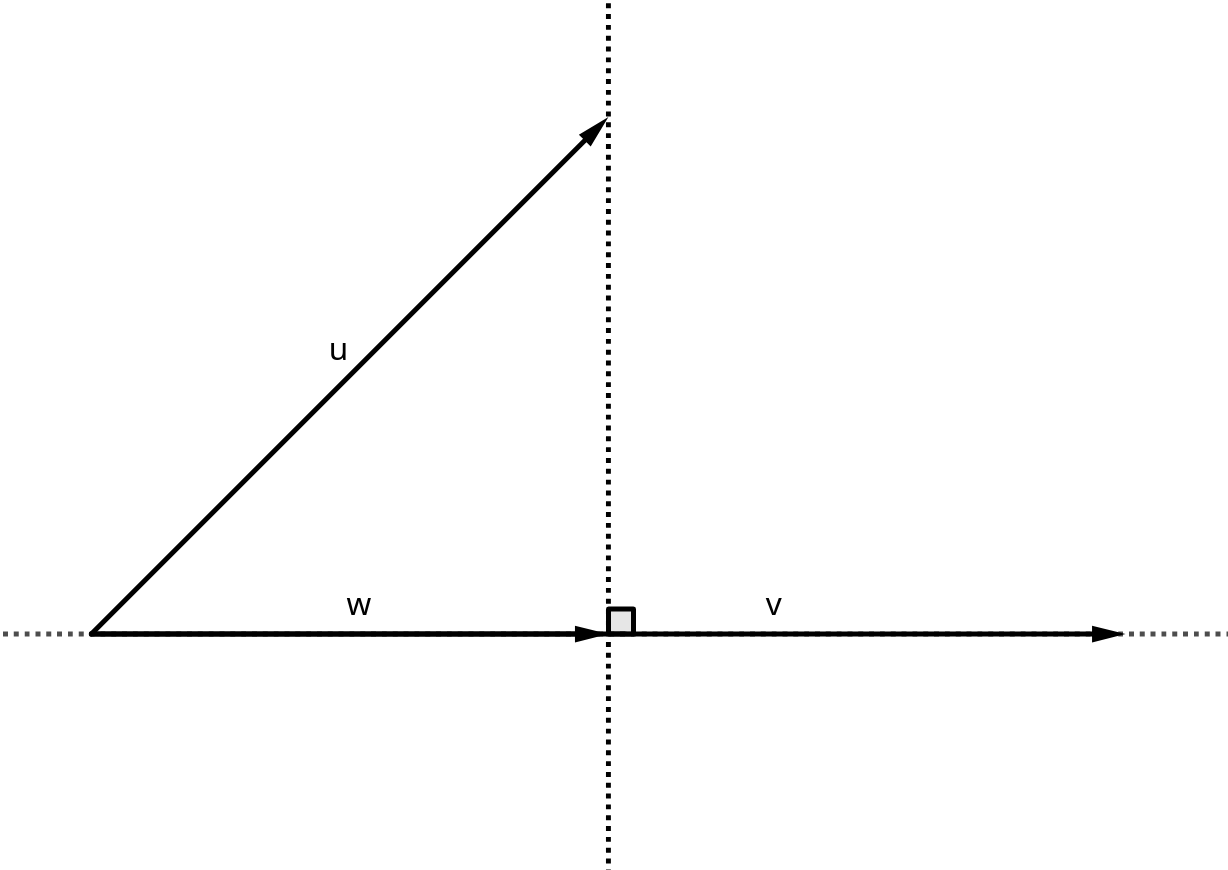
\includegraphics[width=0.75\textwidth]{Figuras/projecao.png}\\
        \footnotesize{Fonte: O autor.}
        \label{fig:projecao}
    \end{figure}

\begin{definition}[combinação linear]
    Seja $V$ um espaço vetorial, dizemos que um vetor $\vec{v}$ é uma combinação linear de outros vetores $\vec{v_1}, \vec{v_2}, \vec{v_3},...,\vec{v_n} \in V$ se e somente se existem escalares $a_1, a_2, a_3,...,a_n \in \mathbb{R}$ tais que $\vec{v}=a_1 \vec{v_1}+a_2 \vec{v_2}+ a_3 \vec{v_3}+...+a_n \vec{v_n}$.
\end{definition}

    \begin{exemplo}
        O vetor $\vec{w} = (5,3) \in \mathbb{R}^{2}$, pode ser escrito como uma combinação linear dos vetores $\vec{u} = (1,0)$ e $\vec{v} = (0,1)$. Isso pode ser visto por $(5,3) = 5(1,0) + 3(0,1)$.
    \qed
    \end{exemplo}

\begin{definition}[dependência e independência linear]
    Seja $V$ um espaço vetorial qualquer e $\vec{v_1}, \vec{v_2}, \vec{v_3},...,\vec{v_n} \in V$, dizemos que o conjunto $\{ \vec{v_1}, \vec{v_2}, \vec{v_3},...,\vec{v_n} \}$ é linearmente independente quando a combinação linear nula $\vec{0}=a_1 \vec{v_1}+a_2 \vec{v_2}+ a_3 \vec{v_3}+...+a_n \vec{v_n}$ implicar que obrigatoriamente $a_1=a_2=a_3=...=a_n= 0$. Caso exista algum escalar $a_n \neq 0$ que satisfaça a combinação linear nula, dizemos que o conjunto $\{ \vec{v_1}, \vec{v_2}, \vec{v_3},...,\vec{v_n} \}$ é linearmente dependente.
\end{definition}

    \begin{exemplo}
        os vetores $\vec{u} = (1,0)$ e $\vec{u} = (0,1)$ são linearmente independentes pois\\

        \begin{center}
            $\begin{array}{rl}
                a_1 (1,0) + a_2 (0,1) &= (0,0)\\
                (a_1,0) + (0,a_2) &= (0,0)\\
                (a_1,a_2) &= (0,0)\\
                a_1 &= 0\\ 
                a_2 &= 0
            \end{array}$
        \end{center}

    \qed
    \end{exemplo}
    
    \begin{exemplo}
        Seja os vetores $\vec{u} = (1,2)$ e $\vec{u} = (3,6)$ do espaço vetorial $\mathbb{R}^{2}$, tais vetores não são linearmente independentes pois,
    
        \begin{center}
            $\begin{array}{rl}
                a_1 (1,2) + a_2 (3,6) &= (0,0)\\
                (a_1,2 a_1) + (3 a_2, 6 a_2) &= (0,0)\\
                (a_1 + 3 a_2, 2 a_1 + 6 a_2) &= (0,0)\\
            \end{array}$
        \end{center}
        
        \begin{center}
            $\begin{cases}
                a_1 + 3 a_2   &= 0\\
                2 a_1 + 6 a_2 &= 0
            \end{cases}$
        \end{center}
    
        \noindent
        resolvendo o sistema acima, encontramos infinitas soluções em que $a_1$ e $a_2$ são diferentes de 0, determinando assim que os vetores $\vec{u} = (1,2)$ e $\vec{u} = (3,6)$ são linearmente dependentes.
    
    \qed
    \end{exemplo}
    
\begin{definition}[base de espaços vetoriais]
    Um conjunto de vetores $\beta = \{ \vec{v_1}, \vec{v_2}, \vec{v_3},...,\vec{v_n} \}$ é considerado uma base para um espaço vetorial $V$, se as seguintes condições forem satisfeitas:
    \begin{itemize}
        \item[(i)] $\beta$ é linearmente independente;
        \item[(ii)] para todo vetor $\vec{v}\in V$ existem $a_1, a_2, \ldots, a_n\in \mathbb{R}$ tal que $\vec{v}=a_1\vec{v_1}+a_2\vec{v_2}+\ldots+a_n\vec{v_n}$.
    \end{itemize}
\end{definition}

\begin{definition}[dimensão de espaços vetoriais]
    A dimensão de um espaço vetorial $V$ é a quantidade de elementos de sua base geradora, denotada por $Dim(V)$.
\end{definition}

\pagebreak
\section{Álgebra abstrata}
\label{ap:abstract_algebra}
Uma operação binária interna é uma função (eventualmente) parcial $\oplus:\mathbb{A}^{2}\rightarrow\mathbb{A}$ e é usualmente denotada como um par ordenado <$\mathbb{A}, \oplus$>, no qual $\mathbb{A}$ é denominado conjunto suporte. A seguir são apresentadas algumas propriedades de operações binárias internas.

\begin{itemize}
    \item[(i)] \textbf{fechada:} $\oplus:\mathbb{A}^{2}\rightarrow\mathbb{A}$ é função total
	\item[(ii)] \textbf{comutativa:} $\forall a,b \in \mathbb{A}\:(a \oplus b = b \oplus a)$
	\item[(iii)] \textbf{associativa:} $\forall a,b \in \mathbb{A}\:((a \oplus b) \oplus c = (c \oplus b) \oplus a = a \oplus b \oplus c)$
	\item[(iv)] \textbf{elemento neutro:} $\exists e \in \mathbb{A}\:\forall a \in \mathbb{A}\:(a \oplus e = a = e \oplus a)$
	\item[(v)] \textbf{elemento inverso:} $\forall a \in \mathbb{A}\:\exists \bar{a} \in \mathbb{A}\:(a \oplus \bar{a} = e = \bar{a} \oplus a)$
\end{itemize}

\begin{definition}[grupoide]
    Um grupoide é um conjunto não vazio junto a uma operação binária fechada. Se um grupoide respeitar a propriedade de comutatividade, denomina-se grupoide abeliano.
\end{definition}

    \begin{exemplo}
         a realização da operação de subtração entre os elementos do conjunto dos inteiros é sempre um inteiro, portanto ($\mathbb{Z},-$) denota um grupoide não abeliano, visto que se $a,b \in \mathbb{Z}\ a - b \neq b - a$. 
    \qed
    \end{exemplo}

\begin{definition}[semigrupo]
    Um semigrupo é definido como um conjunto não vazio que possui uma operação binária fechada e associativa. Se a operação binária também respeitar a propriedade de comutatividade, é dito que o semigrupo é abeliano.
\end{definition}

\begin{definition}[monoide]
    Os monoides são definidos por um conjunto não vazio e uma operação binária que respeita as propriedades de fechamento, associatividade e possui elemento neutro. Se um monoide também possuir a propriedade de comutatividade, é dito que o monoide é abeliano.
\end{definition}

    \begin{exemplo}
         A realização da operação de multiplicação entre os elementos do conjunto $\mathbb{Z}^{*}$ denotam um semigrupo, visto que respeitam a associatividade, portanto ($\mathbb{Z}^{*},*$) é um semigrupo. Entretanto, a estrutura ($\mathbb{Z}^{*},*$) também pode ser classificada como um monoide, pois possui elemento neutro 1 para a operação de multiplicação.
    \qed
    \end{exemplo}
    
    
\begin{definition}[grupo]
    Grupos são definidos como um  conjunto não vazio que possui operação binária que respeita as propriedades de fechamento, associatividade, possui elemento neutro e elemento inverso. Se um grupo respeitar a propriedade de comutatividade, é dito que o grupo é abeliano.
\end{definition}

    \begin{exemplo}
    \label{exemplo:grupo}
        A estrutura ($\mathbb{Z},+$) é um grupo, visto que a operação de soma entre os elementos de $\mathbb{Z}$ possui as propriedades de fechamento, associatividade, possui elemento neutro 0 e possui elemento inverso $a,a' \in \mathbb{Z}\ a + (-a) = 0$. A estrutura ($\mathbb{Z},+$) também possui a propriedade comutativa, sendo assim, classificada como um grupo abeliano. 
    \qed
    \end{exemplo}
    
\begin{definition}[anel]
    Um anel ($A, \oplus, \otimes$) é uma álgebra constituída de um conjunto suporte e duas operações $\oplus$ e $\otimes$ na qual:

    \begin{itemize}
        \item ($A , \oplus$) é um grupo abeliano;
    	\item $\otimes$ é associativo; e
    	\item $\forall a,b,c \in A (a \otimes (b \oplus c)) = ((a \otimes b) \oplus (a \otimes c))$.
    \end{itemize}
\end{definition}

    \begin{exemplo}
        A estrutura ($\mathbb{Z},+,*$) é um anel, pois demonstramos no exemplo \ref{exemplo:grupo} que a estrutura ($\mathbb{Z},+$) é um grupo abeliano, a operação de multiplicação é associativa entre os elementos de $\mathbb{Z}$ e também respeita a distributividade da multiplicação na soma.
    \qed
    \end{exemplo}

    Outros anéis importantes que serão utilizados com frequência neste trabalho são: anel polinomial e anel quociente.
    
\begin{definition}[anel polinomial]
    Sendo o polinômio P na forma $P(x) = a_0 + a_1x^1 + a_2x^2 + ... + a_nx^n$ com $n \in \mathbb{N}$, P é um anel polinomial se seus coeficientes ($a_0, a_1, a_2,...,a_n$) pertencem a um anel A. Denota-se então que $P \in A[x]$.
\end{definition}

\begin{definition}[anel quociente]
    Seja um anel $A$ e um ideal bilateral $I \subseteq A$. Tem-se o anel quociente $A/I$ formado pelo conjunto de todas as classes de equivalência modulo $I$.
\end{definition}

\begin{definition}[classes e relações de equivalência]
    Uma relação $R$ sobre dois elementos $x,y \in A$ denotada por $xRy$, é uma relação de equivalência se satisfazer as seguintes propriedades:

    \begin{itemize}
        \item[(i)] reflexiva: $xRx$
        \item[(ii)] simétrica: $xRy$ então, $yRx$
        \item[(iii)] transitiva: $xRy$ e $yRz$ então $xRz$
    \end{itemize}

    O conjunto de todos os elementos pertencentes a uma relação de equivalência $R$, é conhecido como classe de equivalência de $R$.
\end{definition}

\begin{definition}[ideais]
    Sejam $A$ um anel e $I$ um subconjunto não vazio de $A$.
    Dizemos que $I$ é um ideal à esquerda de $A$ se satisfazer as seguintes propriedades:
    
    \begin{enumerate}
        \item[(i)] se $x, y,  \in I$, então $x-y \in I$ e,
        \item[(ii)] se $a \in A, x \in I$, então $ax \in I$.
    \end{enumerate}
    
    Analogamente define-se um ideal à direita I de $A$ como um subconjunto não vazio tal que:
    
    \begin{enumerate}
        \item[(i)] se $x, y,  \in I$, então $x-y \in I$ e,
        \item[(ii)] se $a \in A, x \in I$, então $xa \in I$.
    \end{enumerate}
    
    Se $I$ é um ideal simultaneamente à direita e à esquerda de $R$ dizemos que $I$ é um ideal (bilateral) de $R$.
\end{definition}

    \begin{exemplo}
         Sendo o anel dos inteiros $\mathbb{Z}$ e o conjunto dos inteiros pares representado por $2\mathbb{Z} \subset \mathbb{Z}$ é um ideal de $\mathbb{Z}$, pois a subtração de qualquer inteiro par por outro inteiro par resulta em um inteiro par, e a multiplicação de um inteiro par por outro inteiro qualquer, resulta em um inteiro par. 
    \qed
    \end{exemplo}

    Outro tipo ideal que deve ser mencionado, é o ideal polinomial na forma $\langle x^{n} + 1 \rangle \subset \mathbb{Z}[x]$. Este ideal representa todos os polinômios múltiplos de $x^{n} + 1$ pertencentes a $\mathbb{Z}[x]$, visto que, sejam $P(x),Q(x) \in \langle x^{n} + 1 \rangle $, $P(x)(x^{n}+1) - Q(x)(x^{n}+1) = (P(x)-Q(x))(x^{n}+1)$ e seja $G(x) \notin \langle x^{n} + 1 \rangle$, $P(x)(x^{n}+1)G(x) = (P(x)G(x))(x^{n}+1)$.

    O anel quociente $\mathbb{Z}_p[x] / \langle x^n+1 \rangle$ é de grande importância para esse trabalho, esta estrutura é utilizada no esquema M-LWE empregado pelo Kyber. Seja $a,b \in \mathbb{Z}_p[x]$, um ideal $\langle x^n+1 \rangle \in \mathbb{Z}_p[x]$ e a relação de equivalência definida por $a \equiv b\ (\textbf{mod}\ \langle x^n+1 \rangle$) se $a - b \in \langle x^n+1 \rangle$. O anel quociente $\mathbb{Z}_p[x] / \langle x^n+1 \rangle$ é uma classe de equivalência formada pelo conjunto de todos os polinômios pertencentes a $\mathbb{Z}_p[x]$ módulo $x^n+1$. Isto é, um polinômio pertencente a $\mathbb{Z}_p[x] / \langle x^n+1 \rangle$ é um polinômio que pertence ao anel $\mathbb{Z}_p[x]$ de grau menor que $n$ com coeficientes entre 0 e $p-1$.

    \begin{exemplo}
    \label{exemplo:soma_em_Z[x]/<I>}
        seja o anel quociente $\mathbb{Z}_7[x] / \langle x^5+1 \rangle$ e os polinômios $a(x) = 5 + 6x + x^3 - 2x^4 - 3x^5 \in \mathbb{Z}_7[x] / \langle x^5+1 \rangle$ e $b(x) = 1 - x + 4x^2 + 3x^4 + x^5 \in \mathbb{Z}_7[x] / \langle x^5+1 \rangle$. A operação de soma entre $a(x)$ e $b(x)$ é definida por:

        \begin{center}
            $\begin{array}{rl}
                c(x) &= a(x) + b(x)\\
                c(x) &= (5 + 6x + x^3 - 2x^4 - 3x^5) + (1 - x + 4x^2 + 3x^4 + x^5)\\
                c(x) &= 6 + 5x + 4x^2 + x^3 + x^4 - 2x^5
            \end{array}$
        \end{center}
    \qed
    \end{exemplo}

    A operação de soma não altera o grau do polinômio resultante, entretanto a multiplicação polinomial altera. Desta forma, para que o resultado pertença ao anel quociente $\mathbb{Z}_7[x] / \langle x^5+1 \rangle$, é necessário realizar uma divisão polinomial onde o resultado é o resto.

    \begin{exemplo}
    \label{exemplo:multiplicacao_em_Z[x]/<I>}
        Sejam os mesmos polinômios do exemplo \ref{exemplo:soma_em_Z[x]/<I>}, a operação de multiplicação entre $a(x)$ e $b(x)$ é definida por:

        \begin{center}
            $\begin{array}{rl}
                c(x) &= a(x) * b(x)\\
                c(x) &= (5 + 6x + x^3 - 2x^4 - 3x^5) * (1 - x + 4x^2 + 3x^4 + x^5)\\
                c(x) &= 5 + x + 14x^2 + 25x^3 + 12x^4 + 26x^5 + x^6 - 9x^7 - 5x^8 - 11x^9 - 3x^{10}\\
                c(x) &= c(x)\ \textbf{mod}\ x^5 + 1\\ 
                c(x) &= -24 + 23x^2 + 30x^3 + 23x^4\\
                c(x) &= (-24\ \textbf{mod}\ 7) + (23\ \textbf{mod}\ 7)x^2 + (30\ \textbf{mod}\ 7)x^3 + (23\ \textbf{mod}\ 7)x^4\\
                c(x) &= 4 + 2x^2 + 2x^3 + 2x^4\\
            \end{array}$
        \end{center}
    
    \qed
    \end{exemplo}
    
    Um polinômio que pertence ao anel quociente $\mathbb{Z}_7[x] / \langle x^5+1 \rangle$ deve possui grau menor que 5 e coeficientes menores que 7. De modo prático, para limitar o grau de um polinômio que exceda grau 5, é realizada a operação \textbf{mod} $x^5 + 1$ sobre este polinômio, e para limitar os coeficientes é realizada a operação \textbf{mod} $7$ em cada coeficiente do polinômio.
    
\begin{definition}[corpos]
    Um corpo $\mathbb{K}$ é um anel comutativo com unidade, ou seja, possui elemento neutro para multiplicação, e todo elemento diferente do elemento neutro da adição (denotado por 0) possui um elemento inverso com relação à multiplicação, isso é $\forall a \in \mathbb{K}-\{0\}, \exists b \in \mathbb{K}$ tal que a.b = b.a = 1.
\end{definition}

    O conjunto dos inteiros módulo $p$, sendo $p$ um número primo, denotado por $\mathbb{Z}_p = \{0,1,2,...,p-1\}$ é um corpo.
    
    \begin{exemplo}
        $\mathbb{Z}_{3} = \{0,1,2\}$ é um corpo, pois $1*1\ \textbf{mod}\ 3=1$ e $2.2\ \textbf{mod}\ 3 = 1$.
    \qed
    \end{exemplo}

    \begin{contraexemplo}
        o conjunto $\mathbb{Z}_{4} = \{0,1,2,3\}$ não é um corpo, pois nenhum número pertencente a $\mathbb{Z}_4-\{0\}$ multiplicado por 2 módulo 4 resulta em 1, ou seja, existe um elemento do conjunto $\mathbb{Z}_4$ que não possui inverso multiplicativo.
    \qed
    \end{contraexemplo}

    \begin{definition}
        Um módulo M sobre um anel unitário A (ou um A-módulo unitário) é um grupo abeliano (M, +) em conjunto com uma operação de um anel unitário A em M, que se escreve $(a, v) \rightarrow av$, satisfazendo as seguintes propriedades \cite{introducao_a_algebra}:

        \begin{enumerate}
            \item[(i)] \ $a(v_1 + v_2) = a v_1 + a v_2, a \in A, v_1 , v_2 \in M$;
            \item[(ii)] \ $(a_1 + a_2)v = a_1 v + a_2 v, a_1, a_2 \in A, v \in M$;
            \item[(iii)] \ $a_1 (a_2 v) = (a_1 a_2)v, a_1, a_2 \in A, v \in M$;
            \item[(iv)] \ $1 v = v, v \in M$.
        \end{enumerate}
    \end{definition}

    Um módulo se assemelha aos espaços vetoriais, com a diferença que os escalares dos espaços vetoriais pertencem a um corpo, enquanto os escalares de um módulo pertencem a um anel.

\pagebreak
\section{Espaços métricos}
\label{sec:espacos_metricos}
    Quando for abordado o conceito de reticulados, estrutura na qual o algoritmo \ac{ML-KEM} é baseado, serão necessários alguns conceitos envolvendo espaços métricos, visto que um reticulado é um espaço métrico. Alguns problemas envolvendo reticulados possuem sua dificuldade de resolução associada a uma métrica, desta forma, vê-se necessário uma introdução sobre espaços métricos.

    Uma métrica em um conjunto $M$ é uma função $d:M \times M \rightarrow \mathbb{R}^{+}$, essa função associa cada par de elementos $x,y \in M$ a um número real positivo $d(x,y)$, chamado distância de x a y. Seja $x,y$ e $z \in M$, a função $d$ precisa satisfazer as seguintes propriedades:

    \begin{enumerate}
        \item[(i)] $d(x,x) = 0$,
        \item[(ii)] Se $x \neq y$ então $d(x,y) > 0$,
        \item[(iii)] $d(x,y) = d(y,x)$ e
        \item[(iv)] $d(x,z) \leq d(x,y) + d(y,z)$.
    \end{enumerate}

    Alguns exemplos de métricas que podem ser utilizada para medir a distância entre dois elementos $x,y$ de um conjunto qualquer são:

    \noindent
    Métrica euclidiana:
    $$d(x,y) = \sqrt{\sum_{i=1}^{n} (x_i - y_i)^2}$$

    \noindent
    Métrica de Manhattan:
    $$d(x,y) = \sum_{i=1}^{n} \vert x_i - y_i \vert$$

    \noindent
    Métrica de Chebyshev:
    $$d(x,y) = \lim_{p \to \infty} \left( \sum_{i=1}^{n} (x_i - y_i)^p \right)^{1/p} $$

    \noindent
    Métrica de Minkowski:
    $$d(x,y) = \left( \sum_{i=1}^{n} (x_i - y_i)^p \right)^{1/p} $$
    
    A métrica de Minkowski, também é conhecida como norma $l_p$, é uma generalização das três métricas anteriores: euclidiana $p = 2$, Manhattan $p = 1$ e com $p$ tendendo ao infinito tem-se a métrica de Chebyshev. 

    \begin{definition}[espaço métrico]
        Um espaço métrico é um par $(M,d)$, onde M é um conjunto e d é uma métrica em M.
    \end{definition}

    \begin{exemplo}
        O espaço euclidiano $\mathbb{R}^n$ é um espaço métrico, onde os elementos de $\mathbb{R}^n$ são pontos $x = (x_1,x_2,...,x_n)$. Com a distância definida pela métrica euclidiana.
    \qed
    \end{exemplo}

    Outras definições importantes que é necessário abordar são os conceitos de bolas e esferas. Seja $a$ um ponto no espaço métrico $M$ e $r > 0$ um número real, definimos:

    \begin{definition}[bola aberta]
         A bola aberta de centro $a$ e raio $r$, é o conjunto de pontos de $M$ cuja distância ao ponto $a$ é menor que $r$. $B(a,r) = \{x \in M\ |\ d(x,a) < r\}$.
    \end{definition}

    \begin{definition}[bola fechada]
        A bola fechada de centro $a$ e raio $r$, é o conjunto de pontos de $M$ cuja distância ao ponto $a$ é menor ou igual à $r$. $B{[}a,r{]} = \{x \in M\ |\ d(x,a) \leq r\}$.
    \end{definition}

    \begin{definition}[esfera]
        A esfera de centro $a$ e raio $r$, é o conjunto de pontos de $M$ cuja distância ao ponto $a$ é igual à $r$. $S(a,r) = \{x \in M\ |\ d(x,a) = r\}$.
    \end{definition}

    A Figura \ref{fig:bola} mostra um exemplo de uma bola no plano com raio 1, contendo todos os pontos em cinza. Já a Figura \ref{fig:esfera} mostra um exemplo de uma esfera de raio 1. Lembrando que pode-se ter bolas e esferas de $n$ dimensões, dependendo do espaço métrico que está sendo utilizado.

    \begin{figure}[htb!]
        \begin{minipage}[c]{0.5\linewidth}
            \centering
            \caption{Bola no plano.}
            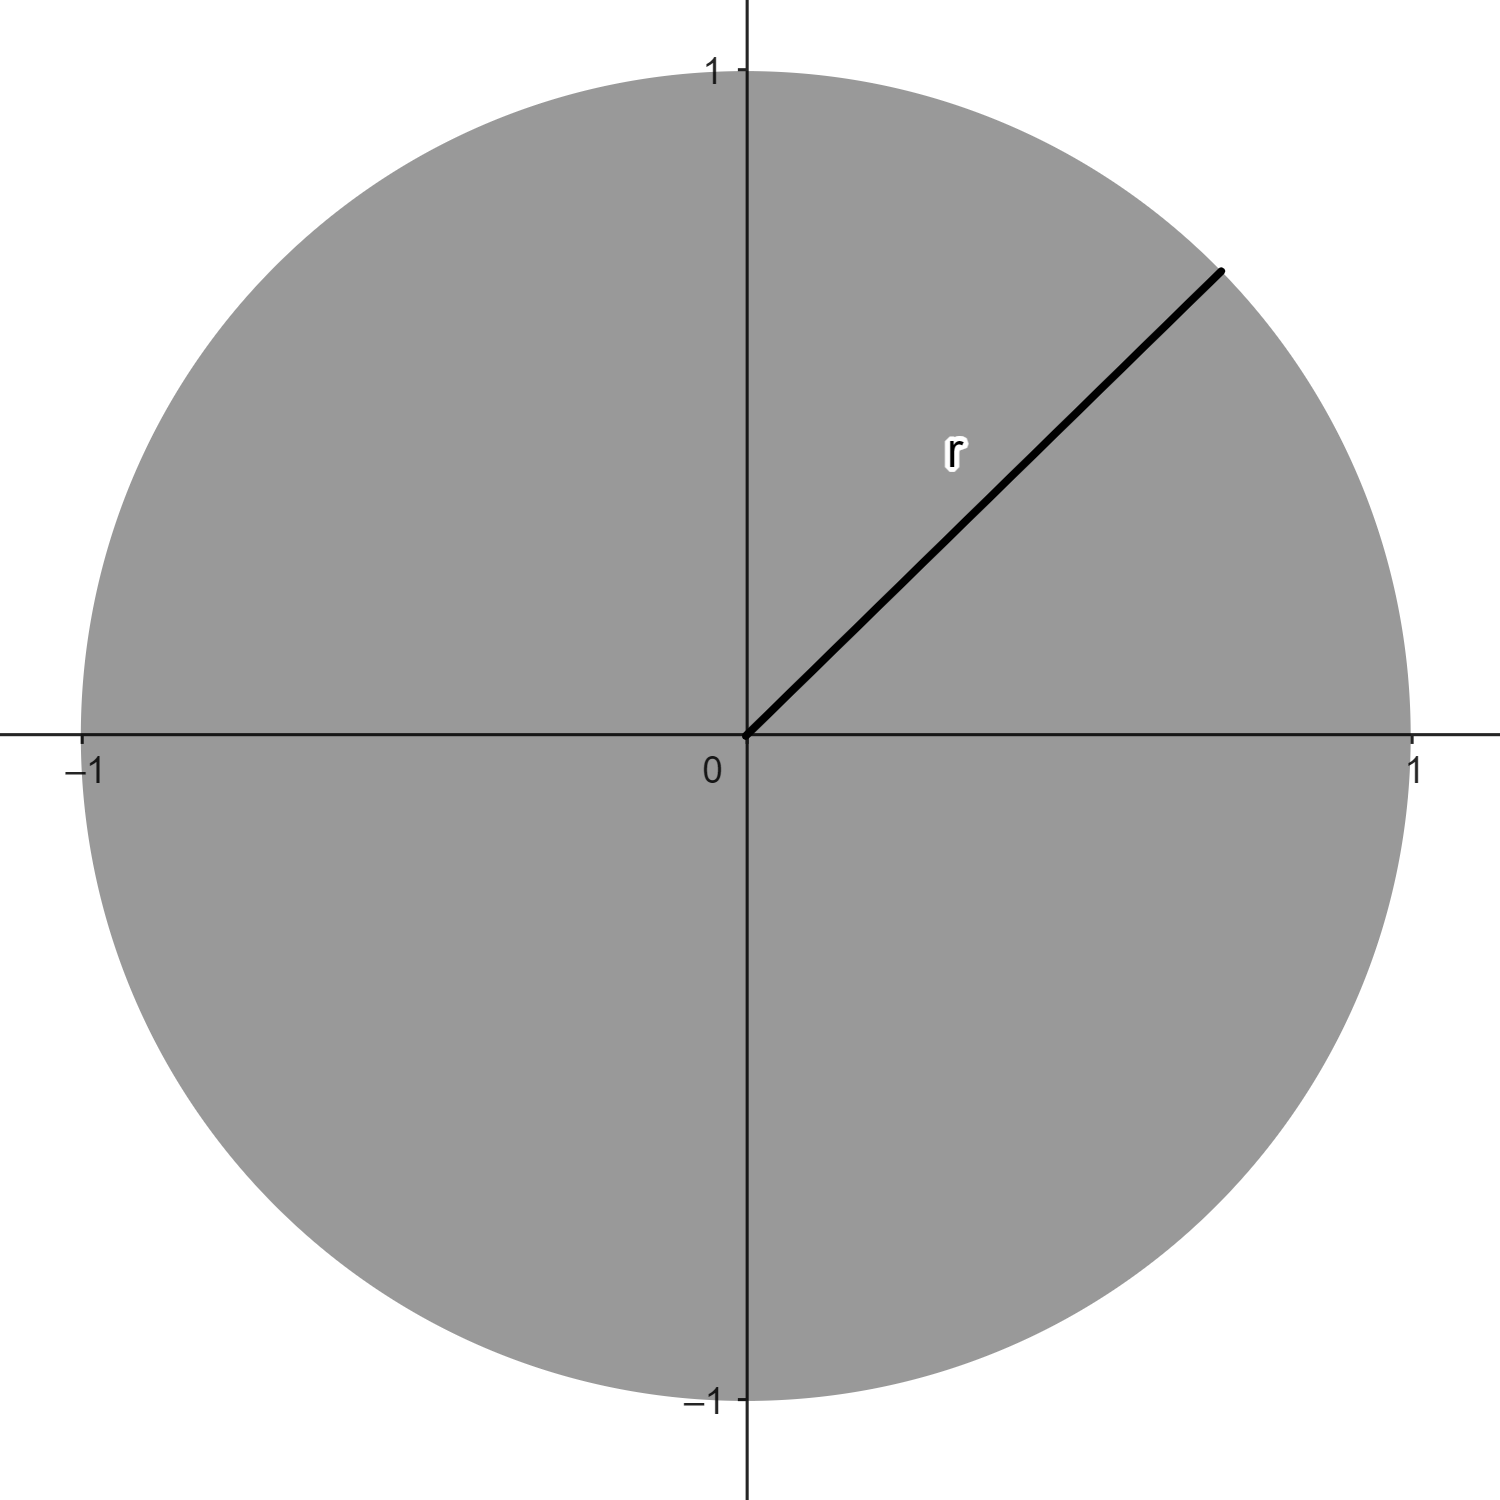
\includegraphics[width=0.75\textwidth]{Figuras/bola.png}\\
            \footnotesize{Fonte: O autor.}
            \label{fig:bola}
        \end{minipage}\hfill
        \begin{minipage}[c]{0.5\linewidth}
            \centering
            \caption{Esfera no plano.}
            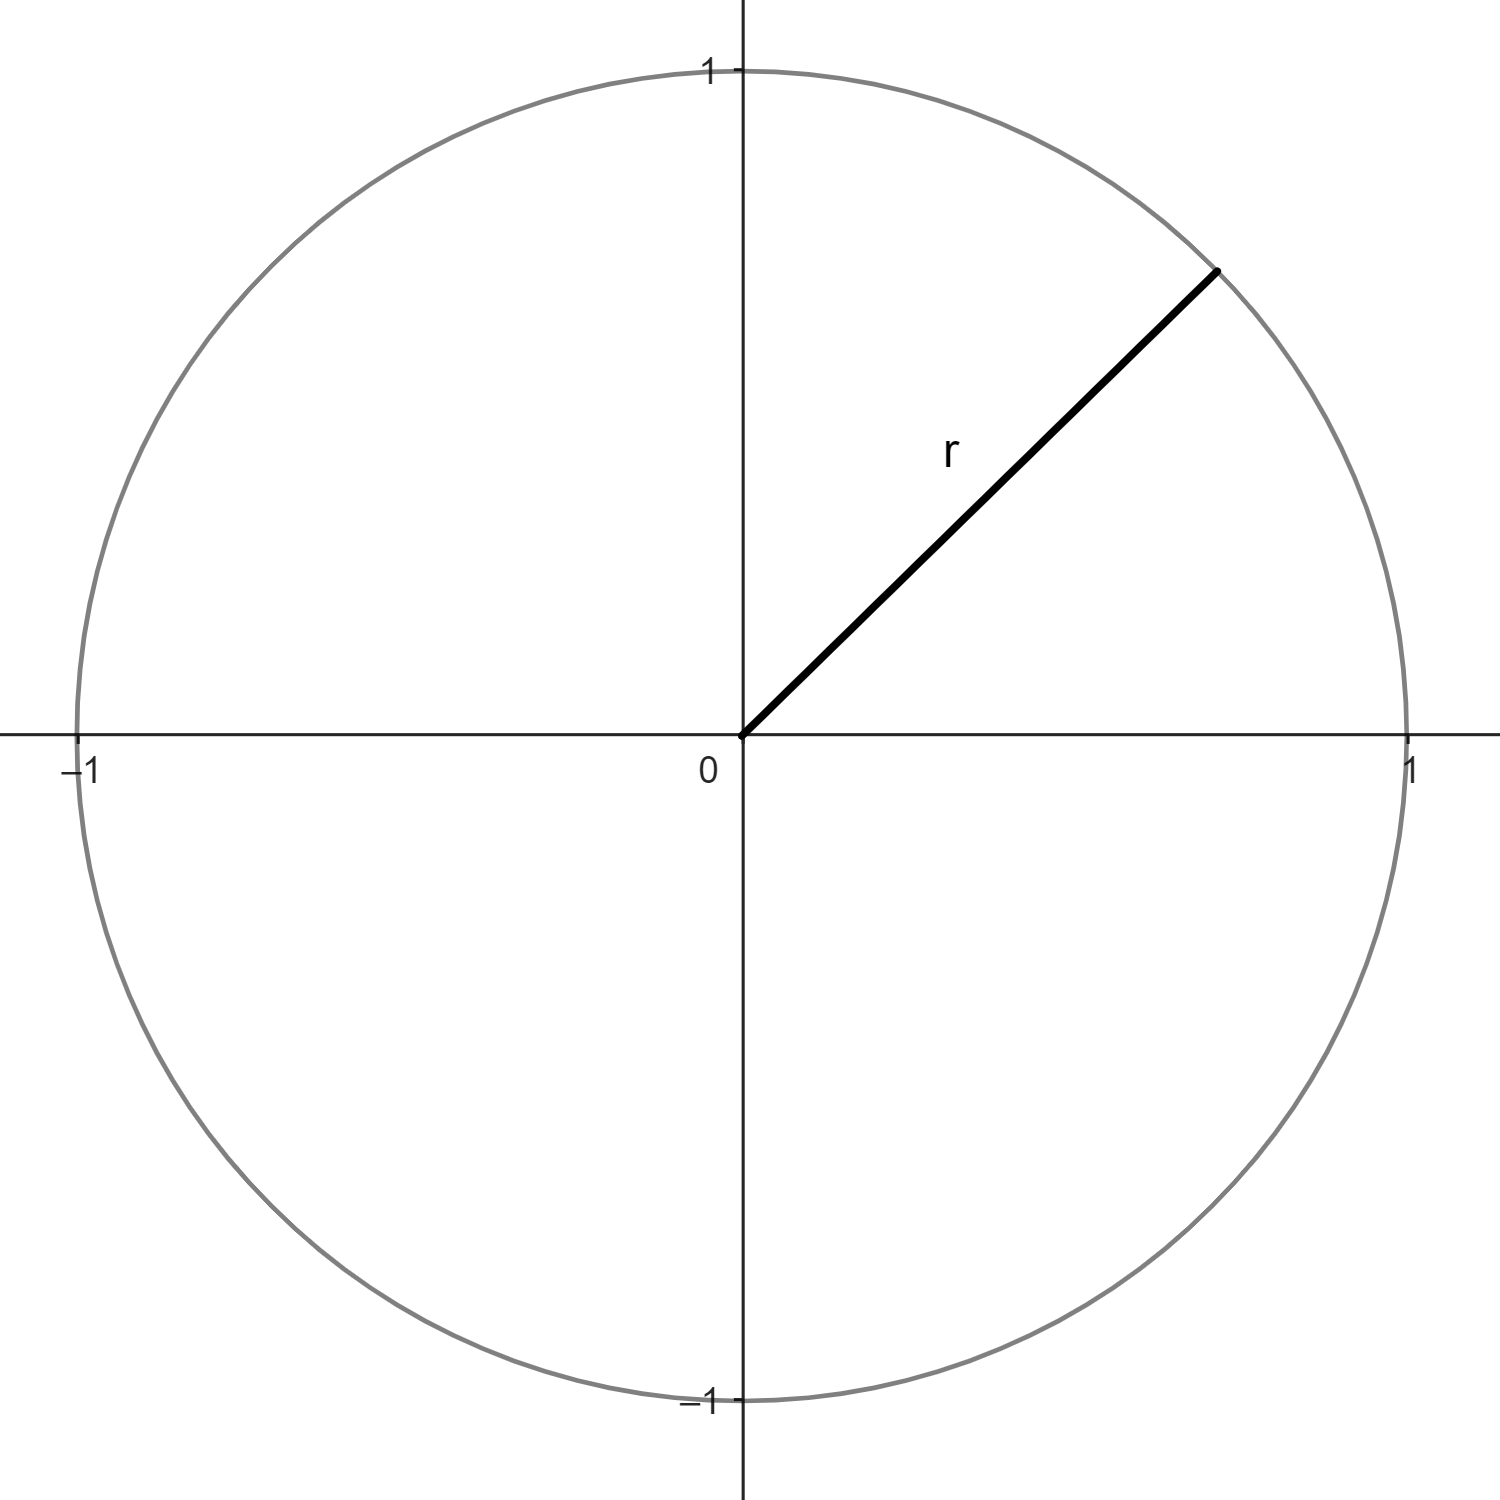
\includegraphics[width=0.75\textwidth]{Figuras/esfera.png}\\
            \footnotesize{Fonte: O autor.}
            \label{fig:esfera}
        \end{minipage}
    \end{figure}

    Seja $a$ um ponto pertencente ao espaço métrico $M$, dizemos que o ponto $a$ é um ponto isolado se $M \cap B(a,r) = \{a\}$, para algum $r > 0$, isto é, se além do próprio ponto $a$, nenhum outro ponto de $M$ está a uma distância inferior a $r$ de $a$.

    \begin{definition}[espaço métrico discreto]
        Um espaço métrico $M$ é dito discreto, se todo elemento pertencente a $M$ for isolado.
    \end{definition}
        
    \begin{exemplo}
        o espaço métrico do conjunto dos inteiros e distância euclidiana é um espaço métrico discreto, pois conseguimos definir um $r > 0$ tal que seja o raio de uma bola aberta com origem em quaisquer inteiro e que este inteiro, seja isolado. Já o conjunto $\{0,1,1/2,...,1/n\}$ não é discreto, pois o elemento 0 não é isolado para algum elemento do conjunto, ou seja, não conseguimos definir uma distância mínima entre os elementos desse conjunto.
    \qed
    \end{exemplo}

\chapter{Demonstrações}
\label{ap:demonstrações}
    Para facilitar a leitura do texto, todas as demonstrações de teoremas e isomorfismos estarão separados neste apêndice.

    \section{Teorema fundamental da aritmética}
        \begin{theorem}[teorema fundamental da aritmética]
            Todo número natural maior que 1 ou é primo, ou pode ser escrito como um produto de números primos.
        \end{theorem}
    
        \begin{proof}\ 
            \begin{enumerate}
                \item [] Por indução em $n$.
                \item \textit{base da indução}: sendo $n = 2$ e como 2 é um número primo, a base está provada.
                \item \textit{hipótese de indução}: sendo um $k \ge 2$ qualquer, supomos que todo $i = 2,3,...,k$ é primo ou um produto de primos.
                \item \textit{passo indutivo}: provar a propriedade para $k+1$. Caso $k+1$ seja número primo, a propriedade é satisfeita. Caso $k+1$ seja número composto então $k+1 = n_1 n_2$ para $1 < n_1 < k+1$ e $1 < n_2 < k+1$. Aplicando a hipótese de indução em $n_1$ e $n_2$, temos que $k+1$ é um produto de primos, satisfazendo a propriedade.
            \end{enumerate}
        \end{proof}

    \pagebreak
    \section{Isomorfismos aditivos sobre reticulados}
        Seja $\sigma_1$ e $\sigma_{1}^{-1}$ os seguintes mapeamentos entre um reticulado de base de tamanho $n$ e polinômios de grau $n-1$.
    
        \begin{center}
            $\begin{array}{rl}
                \sigma_1 &:P[x] \to \mathbb{Z}^n\\
                       &:a_1 + a_2 x + a_3 x^2 + ... + a_{n} x^{n-1} \to (a_1, a_2, a_3, ... , a_{n})
            \end{array}$\\
        
            $\begin{array}{rl}
                \sigma_1^{-1} &:\mathbb{Z}^n \to P[x]\\
                       &:(a_1, a_2, a_3, ... , a_{n}) \to a_1 + a_2 x + a_3 x^2 + ... + a_{n} x^{n-1}
            \end{array}$\\
        \end{center}
    
        Para provar que de fato $\sigma_1$ é um isomorfismo aditivo, deve-se demonstrar três propriedades:
    
        \begin{itemize}
            \item[(i)] $\sigma_1(P[x] + Q[x]) = \sigma_1(P[x]) + \sigma_1(Q[x])$,
            \item[(ii)] $\sigma_1(\sigma_1^{-1}) = \mathbb{Z}^n$ e
            \item[(ii)] $\sigma_1^{-1}(\sigma_1) = P[x]$.
        \end{itemize}
    
        Demonstração do item (i):\\
        \begin{tabular}{l}
            $\begin{array}{rl}
                 \sigma_1((a_1 + a_2 x + a_3 x^2 + ... + a_{n} x^{n-1}) + (b_1 + b_2 x + b_3 x^2 + ... + b_{n} x^{n-1}))         &= \\ \sigma_1(a_1 + a_2 x + a_3 x^2 + ... + a_{n} x^{n-1}) + \sigma_1(b_1 + b_2 x + b_3 x^2 + ... + b_{n} x^{n-1})\\\\
    
                 \sigma_1((a_1 + b_1) + (a_2 + b_2) x + (a_3 + b_3) x^2 + ... + (a_{n} + b_{n}) x^{n-1}) &=\\ \sigma_1(a_1 + a_2 x + a_3 x^2 + ... + a_{n} x^{n-1}) + \sigma_1(b_1 + b_2 x + b_3 x^2 + ... + b_{n} x^{n-1})\\\\
            
                (a_1 + b_1, a_2 + b_2, a_3 + b_3, ... , a_n + b_n) &=\\ (a_1, a_2, a_3, ... , a_n) + (b_1, b_2, b_3, ... , b_n)\\\\
            
                (a_1 + b_1, a_2 + b_2, a_3 + b_3, ... , a_n + b_n) &=\\ (a_1 + b_1, a_2 + b_2, a_3 + b_3, ... , a_n + b_n)
            
            \end{array}$
        \end{tabular}\\\\
    
        Demonstração do item (ii):\\
        \begin{tabular}{l}
            $\begin{array}{rl}
                \sigma_1(\sigma_1^{-1}(a_1, a_2, a_3, ... , a_n)) &= (a_1, a_2, a_3, ... , a_n)\\
            
                \sigma_1(a_1 + a_2 x + a_3 x^2 + ... + a_{n} x^{n-1}) &= (a_1, a_2, a_3, ... , a_n)\\
                
                (a_1, a_2, a_3, ... , a_n) &= (a_1, a_2, a_3, ... , a_n)\\
            \end{array}$
        \end{tabular}\\\\
    
        Demonstração do item (iii):\\
        \begin{tabular}{l}
            $\begin{array}{rl}
                \sigma_1^{-1}(\sigma_1(a_1 + a_2 x + a_3 x^2 + ... + a_{n} x^{n-1})) &= a_1 + a_2 x + a_3 x^2 + ... + a_{n} x^{n-1}\\
                \sigma_1^{-1}((a_1, a_2, a_3, ... , a_n)) &= a_1 + a_2 x + a_3 x^2 + ... + a_{n} x^{n-1}\\
                a_1 + a_2 x + a_3 x^2 + ... + a_{n} x^{n-1} &= a_1 + a_2 x + a_3 x^2 + ... + a_{n} x^{n-1}
            \end{array}$
        \end{tabular}\\\\
    
        Desta forma provamos que $\sigma_1$ é um isomorfismo aditivo, isto significa que $P[x]$ e $\mathbb{Z}^n$ se comportam da mesma forma com relação à operação de adição.
        Seja $\sigma_2$ e $\sigma_{2}^{-1}$ os seguintes mapeamentos entre um reticulado de base de tamanho $n$ e matrizes-linha com $n$ colunas.
    
        \begin{center}
            $\begin{array}{rl}
                    \sigma_2 &:M_n \to \mathbb{Z}^n\\
                           &:[a_1\ a_2\ a_3\ ...\ a_n] \to (a_1, a_2, a_3, ... , a_n)
            \end{array}$\\
        
            $\begin{array}{rl}
                    \sigma_2^{-1} &:\mathbb{Z}^n \to M_n\\
                           &:(a_1, a_2, a_3, ... , a_n) \to [a_1\ a_2\ a_3\ ...\ a_n]
            \end{array}$\\
        \end{center}
    
        Para provar que $\sigma_2$ é um isomorfismo aditivo, devemos garantir as mesmas três propriedades que provamos para $\sigma_1$, mas agora respeitando o domínio e contradomínio de $\sigma_2$.
    
        Demonstração do item (i):\\
        \begin{tabular}{l}
            $\begin{array}{rl}
                 \sigma_2([a_1\ a_2\ a_3\ ...\ a_n] + [b_1\ b_2\ b_3\ ...\ b_n]) &=  \sigma_2([a_1\ a_2\ a_3\ ...\ a_n]) + \sigma_2([b_1\ b_2\ b_3\ ...\ b_n])\\
                 \sigma_2([a_1 + b_1\ a_2 + b_2\ a_3 + b_3\ ...\ a_n + b_n]) &=  \sigma_2([a_1\ a_2\ a_3\ ...\ a_n]) + \sigma_2([b_1\ b_2\ b_3\ ...\ b_n])\\
                 (a_1 + b_1, a_2 + b_2, a_3 + b_3, ... , a_n + b_n) &= (a_1, a_2, a_3, ... , a_n) + (b_1, b_2, b_3, ... , b_n)\\
                 (a_1 + b_1, a_2 + b_2, a_3 + b_3, ... , a_n + b_n) &= (a_1 + b_1, a_2 + b_2, a_3 + b_3, ... , a_n + b_n)
            \end{array}$
        \end{tabular}\\\\
    
        Demonstração do item (ii):\\
        \begin{tabular}{l}
            $\begin{array}{rl}
                \sigma_2(\sigma_2^{-1}((a_1, a_2, a_3, ... , a_n))) &= (a_1, a_2, a_3, ... , a_n)\\
                \sigma_2([a_1\ a_2\ a_3\ ...\ a_n]) &= (a_1, a_2, a_3, ... , a_n)\\
                (a_1, a_2, a_3, ... , a_n) &= (a_1, a_2, a_3, ... , a_n)\\
            \end{array}$
        \end{tabular}\\\\
    
        Demonstração do item (iii):\\
        \begin{tabular}{l}
            $\begin{array}{rl}
                \sigma_2^{-1}(\sigma_2([a_1\ a_2\ a_3\ ...\ a_n])) &= {[}a_1\ a_2\ a_3\ ...\ a_n{]}\\
                \sigma_2^{-1}((a_1, a_2, a_3, ... , a_n)) &= {[}a_1\ a_2\ a_3\ ...\ a_n{]}\\
                {[}a_1\ a_2\ a_3\ ...\ a_n{]} &= {[}a_1\ a_2\ a_3\ ...\ a_n{]}\\
            \end{array}$
        \end{tabular}\\\\